\chapter{Wstęp}
\label{ch:wstep}

\section{Cel i zakres pracy}
Przedmiotem niniejszej pracy jest przegląd metod wykorzystywanych do planowania bezkolizyjnych tras dla wielu robotów mobilnych.
Stanowi to również wstęp teoretyczny do zaprojektowania algorytmu i implementacji oprogramowania pozwalającego na symulację działania skutecznego planowania tras dla systemu wielorobotowego.

Praca skupia się na przypadkach, w których mamy do czynienia ze środowiskiem z dużą liczbą przeszkód (np. zamknięty budynek z licznymi ciasnymi korytarzami), aby uwypuklić  problem blokowania sią agentów często prowadzący do zakleszczenia. Często okazuje się, że należy wtedy zastosować nieco inne podejścia niż te, które sprawdzają się w przypadku otwartych środowisk, a które zostały opisane np. w pracach \cite{roszkowska}, \cite{siemiatkowska}.
W otwartych środowiskach z małą liczbą przeszkód wystarczające może się okazać np. proste replanowanie wykorzystujące algorytm D* (por. \ref{ch:dstar}) lub LRA* (por. \ref{ch:lra}).

W niniejszej pracy starano się znaleźć metody rozwiązujące zagadnienie, w którym znane są:
\vspace{-1em}
\begin{itemize}[noitemsep]
	\item pełna informacja o mapie otoczenia (położenie statycznych przeszkód),
	\item aktualne położenie i położenie celu każdego z robotów.
\end{itemize}
Szukany jest natomiast przebieg tras do punktów docelowych dla agentów. Zadaniem algorytmu będzie wyznaczenie możliwie najkrótszej bezkolizyjnej trasy dla wszystkich robotów. Należy jednak zaznaczyć, że priorytetem jest dotarcie każdego z robotów do celu bez kolizji z innymi robotami. Drugorzędne zaś jest, aby wyznaczone drogi były możliwie jak najkrótsze.

\clearpage
\subsection{Założenia}
\label{ch:zalozenia}
Założenia i ograniczenia rozważanego problemu:
\begin{enumerate}
	\item Każdy z robotów ma wyznaczony inny punkt docelowy, do którego zmierza.
	\item Planowanie tras dotyczy mobilnych robotów holonomicznych.
	\item Czas trwania zmiany kierunku robota jest pomijalnie mały.
	\item Srodowisko, w którym poruszają się roboty, jest dwuwymiarową przestrzenią zawierającą dużą liczbę przeszkód oraz wąskie korytarze (por. rys. \ref{fig:img_robopath_sample-maze}).
	\item Roboty "wiedzą" o sobie i mogą komunikować się ze sobą podczas planowania tras.
	\item Każdy robot zajmuje w przestrzeni jedno pole. Na jednym polu może znajdować się maksymalnie jeden robot (por. rys. \ref{fig:img_robopath_sample-maze}).
	\item Planowanie tras powinno odbywać się w czasie rzeczywistym.
\end{enumerate}

\begin{figure}[H]
	\centering
	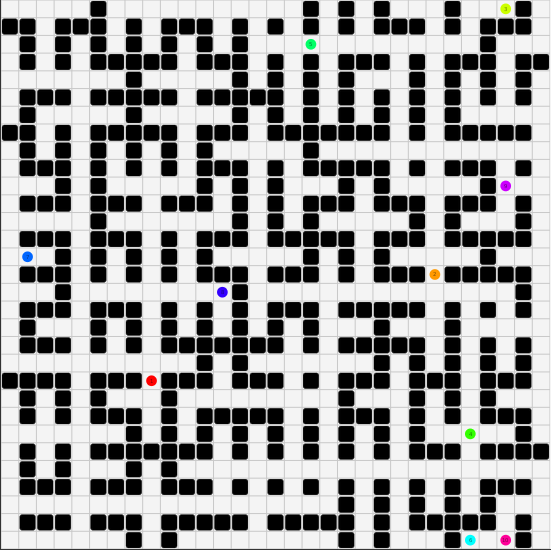
\includegraphics[width=8cm]{img/robopath/sample-maze}
	\caption{Przykładowe środowisko z dużą liczbą przeszkód i rozmieszczonymi robotami. Źródło: własna implementacja oprogramowania symulacyjnego}
	\label{fig:img_robopath_sample-maze}
\end{figure}


\clearpage
\section{Koordynacja ruchu robotów}
Koordynacja ruchu robotów jest jednym z fundamentalnych problemów w systemach wielorobotowych \cite{optpriorities}.

Kooperacyjne znajdowanie tras (ang. {\it Cooperative Pathfinding}) jest zagadnieniem planowania w układzie wieloagentowym, w którym to agenci mają za zadanie znaleźć bezkolizyjne drogi do swoich, osobnych celów. Planowanie to odbywa się w oparciu o pełną informację o środowisku oraz o trasach pozostałych agentów \cite{cooppath}.

Algorytmy do wyznaczania bezkolizyjnych tras dla wielu agentów (robotów) mogą znaleźć zastosowanie w szpitalach (np. roboty TUG i HOMER do dostarczania sprzętu na wyposażeniu szpitala \cite{tughomer}) oraz magazynach (np. roboty transportowe w magazynach firmy Amazon - por. rys. \ref{fig:image_kiva_amazon}).

\begin{figure}[H]
	\centering
	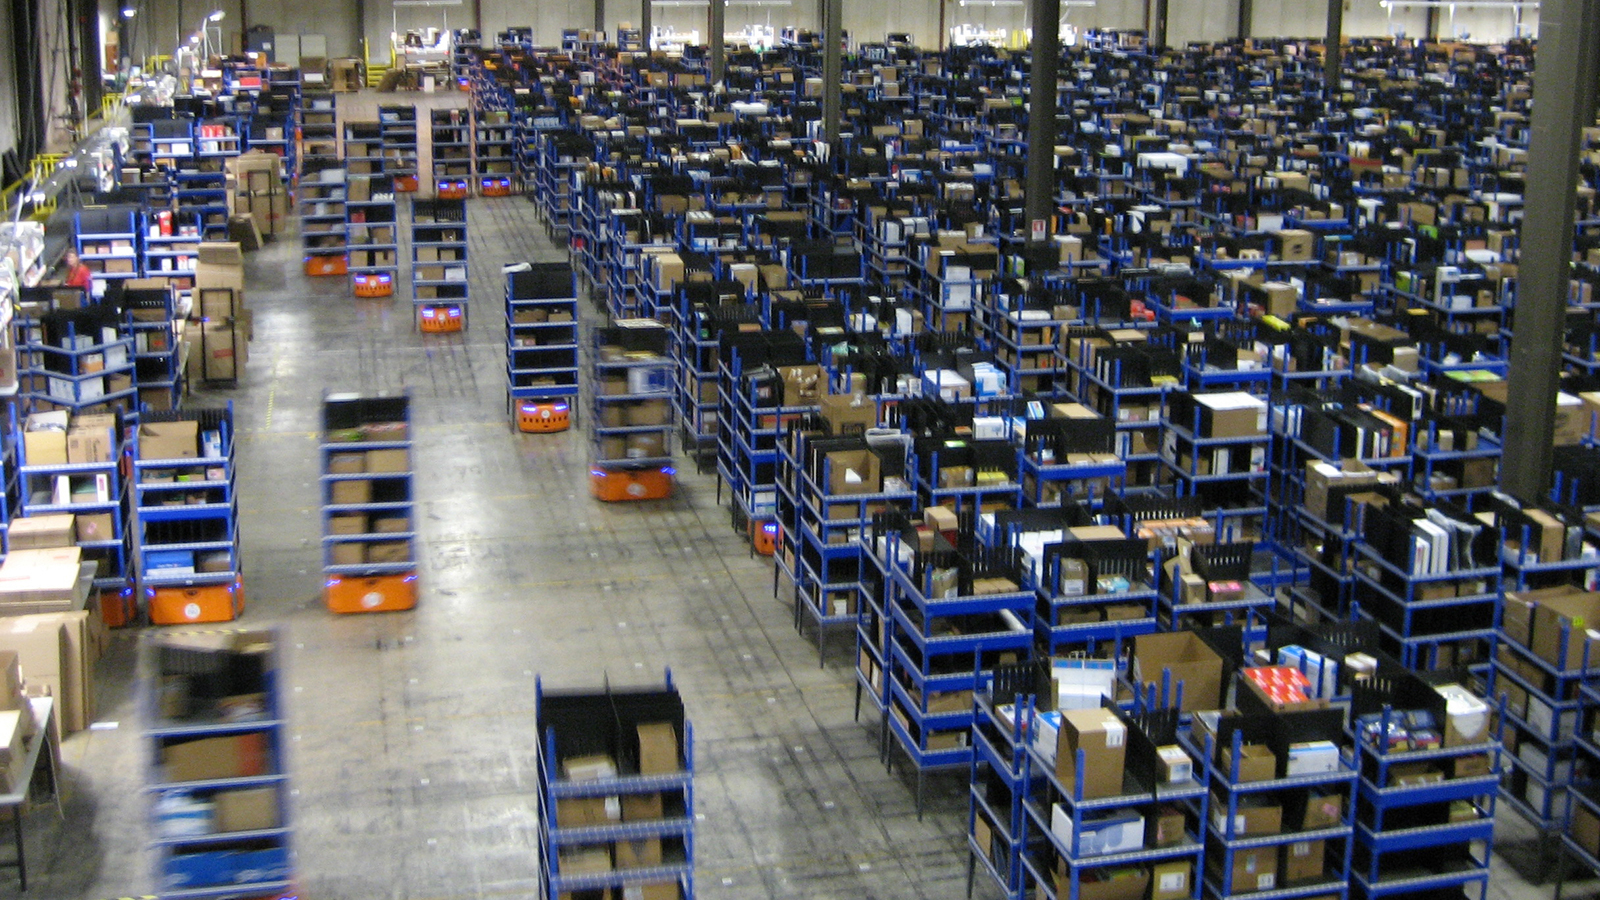
\includegraphics[width=14cm]{img/kiva-amazon}
	\caption{Roboty Kiva pracujące w magazynie firmy Amazon. Źródło: \cite{amazonkiva}}
	\label{fig:image_kiva_amazon}
\end{figure}

\subsection{Podobieństwo do gier RTS}
Problem kooperacyjnego znajdowania tras pojawia się nie tylko w robotyce, ale jest również popularny m.in. w grach komputerowych (strategiach czasu rzeczywistego), gdzie konieczne jest wyznaczanie bezkolizyjnych dróg dla wielu jednostek, unikając wzajemnego blokowania się. Niestety brak wydajnych i skutecznych algorytmów planowania dróg można zauważyć w wielu grach typu RTS (ang. {\it Real-Time Strategy}), gdzie czasami obserwuje się zjawisko zakleszczenia jednostek w wąskich gardłach (np. Age of Empires II, Warcraft III lub nawet we współczesnych produkcjach) \cite{efficient_coop_pathplanning} (por. rys. \ref{fig:img_games_age-deadlock}). Ponadto, zauważalny brak ogólnie dostępnych bibliotek open-source do rozwiązania problemu typu {\it Cooperative Pathfinding} świadczy o potrzebie rozwoju tych metod.

Często algorytmy wykorzystywane w grach typu RTS (ang. {\it Real-Time Strategy}) zajmują się planowaniem bezkolizyjnych dróg dla układu wielu agentów w czasie rzeczywistym (będącego przedmiotem niniejszej pracy), dlatego nic nie stoi na przeszkodzie, aby stosować je zamiennie również do koordynacji ruchu zespołu robotów mobilnych.

\begin{figure}[H]
	\centering
	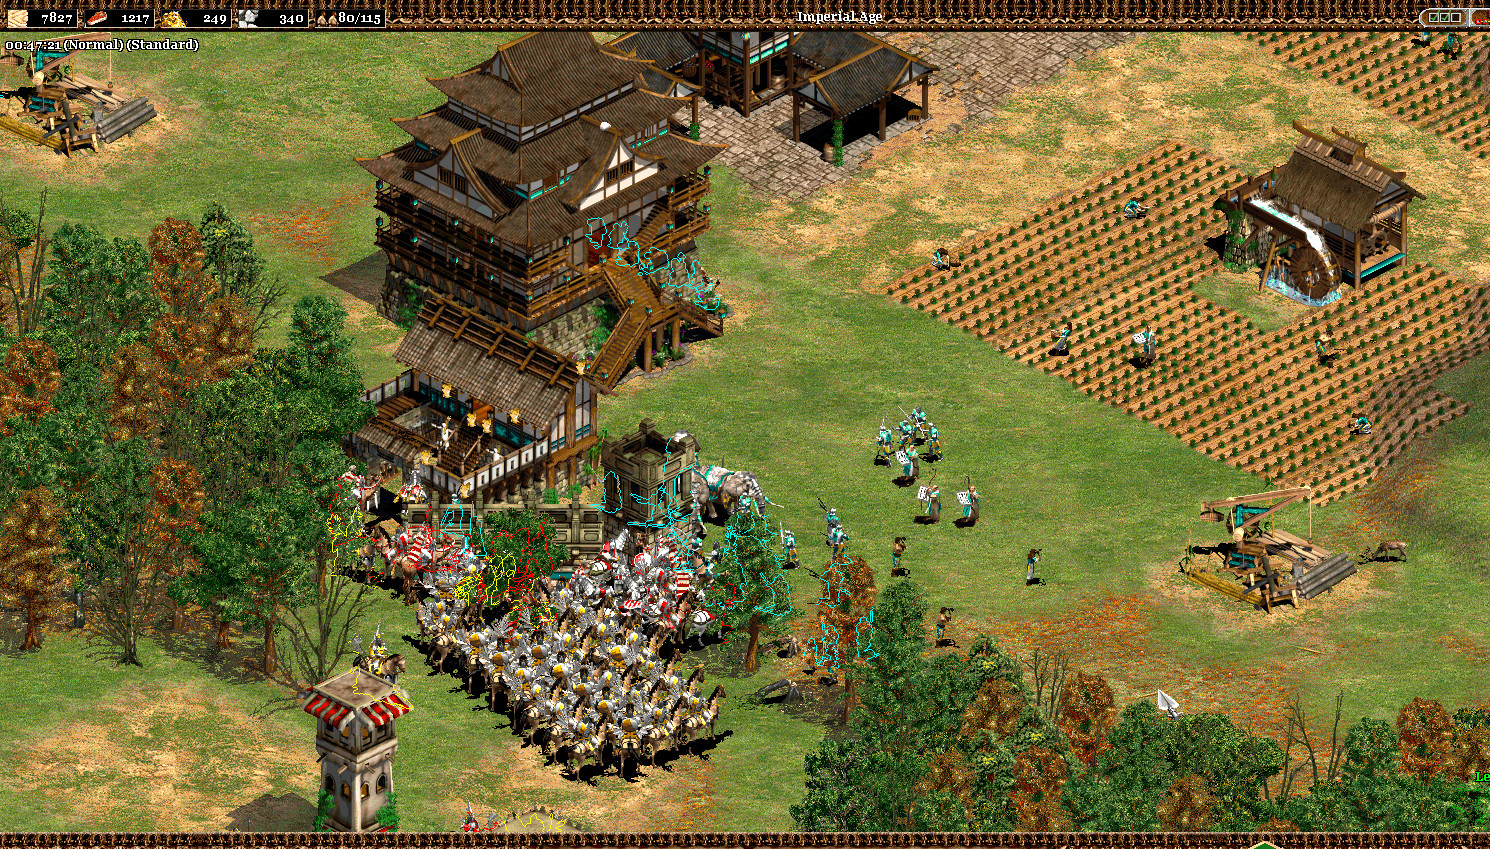
\includegraphics[width=13cm]{img/games/age-deadlock2}
	\caption{Popularny problem zakleszczania się jednostek w wąskich gardłach występujący w grach typu RTS. Źródło: gra komputerowa Age of Empires II Forgotten Empires}
	\label{fig:img_games_age-deadlock}
\end{figure}

\section{Podstawowe pojęcia}
\subsubsection{Robot holonomiczny}
Robot holonomiczny to taki robot mobilny, który może zmienić swoją orientację, stojąc w miejscu.

\subsubsection{Przestrzeń konfiguracyjna}
Przestrzeń konfiguracyjna to $N$-wymiarowa przestrzeń będąca zbiorem możliwych stanów danego układu fizycznego.
Wymiar przestrzeni zależy od rodzaju i liczby wyróżnionych parametrów stanu.
W odróżnieniu od przestrzeni roboczej, gdzie robot ma postać bryły, w przestrzeni konfiguracyjnej robot jest reprezentowany jako punkt.

\subsubsection{Zupełność algorytmu (ang. {\it Completeness})}
W kontekście algorytmu przeszukiwania grafu algorytm zupełny to taki, który gwarantuje znalezienie rozwiązania, jeśli takie istnieje.
Warto zaznaczyć, że nie gwarantuje to wcale, że znalezione rozwiązanie będzie rozwiązaniem optymalnym.

% TODO-MGR
% \subsubsection{Metoda hill-climbing}
% Metoda hill-climbing jest rodzajem matematycznej optymalizacji, lokalną metodą przeszukiwania.
% Jest to iteracyjny algorytm, który zaczyna w wybranym rozwiązaniu problemu, następnie próbuje znaleźć lepsze rozwiązanie poprzez przyrostowe zmiany pojedynczych elementów rozwiązania.
% Jeśli przyrostowa zmiana przynosi lepsze rozwiązanie, jest ona wprowadzana do nowego rozwiązania.
% Kroki algorytmu powtarzane są dotąd, aż żadna zmiana nie przynosi już poprawy.
